\documentclass[11pt]{article}

\usepackage[a4paper,margin=2.5cm]{geometry}
\usepackage{graphicx}
\usepackage{tikz}
\usetikzlibrary{shapes.geometric,arrows.meta,positioning}
\usepackage{listings}
\usepackage{xcolor}
\usepackage{booktabs}
\usepackage[hidelinks]{hyperref}
\usepackage{amsmath}

\definecolor{codebg}{RGB}{245,245,245}
\definecolor{codecomment}{RGB}{110,110,110}
\definecolor{codekeyword}{RGB}{0,0,150}

\lstdefinestyle{code}{
  backgroundcolor=\color{codebg},
  basicstyle=\ttfamily\small,
  commentstyle=\color{codecomment}\itshape,
  keywordstyle=\color{codekeyword}\bfseries,
  numbers=left,
  numberstyle=\tiny\color{gray},
  frame=single,
  breaklines=true,
  showstringspaces=false,
  tabsize=2,
  language=C++
}
\lstset{style=code}

\title{3D Embedded Scanner}
\author{Yuval Rubin \\ David Khutsishvili}
\date{}

\begin{document}

\maketitle
\tableofcontents
\newpage

%==================================================================
\section{Introduction}
%==================================================================

The goal of this project was to build a 3D scanner from
readily available components: an Arduino microcontroller, two
time-of-flight (ToF) distance sensors, and a set of servos. Rather
than moving the sensors around the object, the sensors were fixed in place
on two pillars and the object itself was moved: it sat on a plate that
rotated a full turn at a fixed elevation, and was then stepped down before
rotating again. Sweeping the object through the fixed sensors' line of
sight this way traced out a ring of distance samples over the surface of
the object, in cylindrical coordinates $(\theta, h, r)$.

The core of the project was the embedded system: an Arduino sketch
that sequenced the sensors and actuators and drove the entire scanning
process, streaming raw measurements over serial as they were taken. A
small Python toolchain on the host computer supported this by capturing
that serial stream to a file and reconstructing a 3D point cloud from it,
which was rendered for inspection.

%==================================================================
\section{System Design}
%==================================================================

\subsection{Architecture Overview}

The system was split into two halves that only communicated over a serial
(USB) link: the embedded scanner, which physically performed the scan, and
a host-side Python toolchain, which captured and visualized the resulting
data. Figure~\ref{fig:architecture} shows the overall data and control
flow.

\begin{figure}[h]
  \centering
  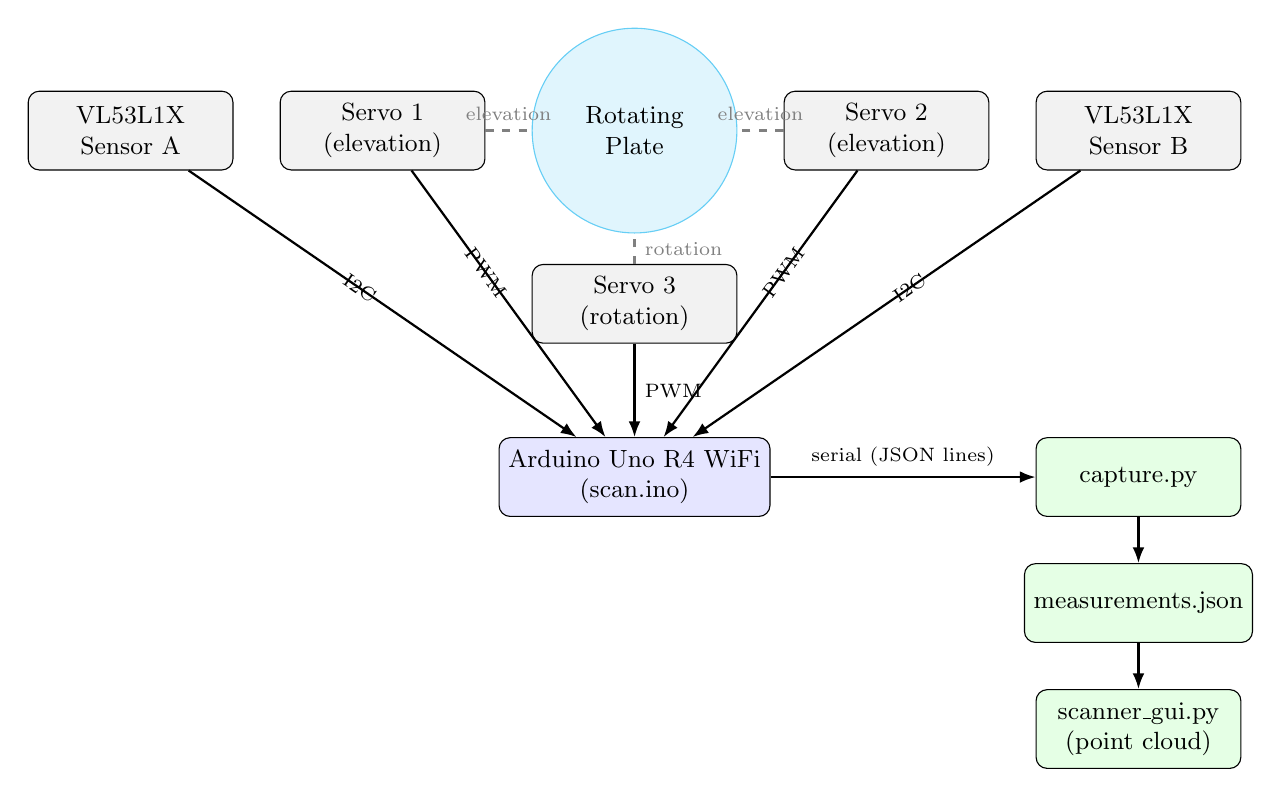
\begin{tikzpicture}[
      box/.style={draw, rounded corners, minimum width=2.6cm, minimum height=1cm, align=center, font=\small},
      dev/.style={box, fill=gray!10},
      mcu/.style={box, fill=blue!10},
      host/.style={box, fill=green!10},
      plate/.style={circle, draw=cyan!60, fill=cyan!12, minimum size=2.6cm, align=center, font=\small},
      arr/.style={-{Latex[length=2mm]}, thick},
      mech/.style={dashed, thick, gray}
    ]
    % Physical layout: left to right, matching how the parts actually
    % sit on the bench.
    \node[dev]   (tofA)   at (0,0)     {VL53L1X\\Sensor A};
    \node[dev]   (servo1) at (3.2,0)   {Servo 1\\(elevation)};
    \node[plate] (plate)  at (6.4,0)   {Rotating\\Plate};
    \node[dev]   (servo2) at (9.6,0)   {Servo 2\\(elevation)};
    \node[dev]   (tofB)   at (12.8,0)  {VL53L1X\\Sensor B};

    \node[dev]   (servo3) at (6.4,-2.2) {Servo 3\\(rotation)};
    \node[mcu]   (mcu)    at (6.4,-4.4) {Arduino Uno R4 WiFi\\(scan.ino)};

    \node[host] (capture) at (12.8,-4.4) {capture.py};
    \node[host] (json)    at (12.8,-6.0) {measurements.json};
    \node[host] (gui)     at (12.8,-7.6) {scanner\_gui.py\\(point cloud)};

    % mechanical couplings (how the servos actually move the plate)
    \draw[mech] (servo1) -- node[midway, above, font=\scriptsize]{elevation} (plate);
    \draw[mech] (servo2) -- node[midway, above, font=\scriptsize]{elevation} (plate);
    \draw[mech] (servo3) -- node[midway, right, font=\scriptsize]{rotation} (plate);

    % electrical / data connections into the Arduino
    \draw[arr] (tofA)   -- node[left, sloped, font=\scriptsize]{I2C} (mcu);
    \draw[arr] (tofB)   -- node[right, sloped, font=\scriptsize]{I2C} (mcu);
    \draw[arr] (servo1) -- node[left, sloped, font=\scriptsize]{PWM} (mcu);
    \draw[arr] (servo2) -- node[right, sloped, font=\scriptsize]{PWM} (mcu);
    \draw[arr] (servo3) -- node[right, font=\scriptsize]{PWM} (mcu);

    \draw[arr] (mcu) -- node[above, font=\scriptsize]{serial (JSON lines)} (capture);
    \draw[arr] (capture) -- (json);
    \draw[arr] (json) -- (gui);
  \end{tikzpicture}
  \caption{System architecture, laid out to match the physical bench
    arrangement: sensor A, servo 1, the rotating plate, servo 2, and
    sensor B sit side by side, with servo 3 driving the plate's rotation
    from below. The Arduino drove all five devices directly and streamed
    JSON measurement lines over serial; the host captured them to a file
    and turned them into a point cloud.}
  \label{fig:architecture}
\end{figure}

\subsection{Microcontroller}

The scanner was controlled by an \textbf{Arduino Uno R4 WiFi}. Only its
standard digital I/O, PWM, and I2C peripherals were used (WiFi was not
used by the project). It was responsible for:
\begin{itemize}
  \item bringing up and reading both distance sensors over I2C,
  \item driving the three servos over PWM,
  \item sequencing the scan (elevation rings, rotation steps),
  \item streaming measurements to the host as line-delimited JSON over the
    serial (USB) connection.
\end{itemize}

\subsection{Sensors}

Two \textbf{Adafruit VL53L1X} time-of-flight distance sensors were mounted a
fixed distance apart (\texttt{SENSOR\_DIST}) on two static pillars, aimed
inward toward the object. Using two sensors instead of one let the system
sample two points on the object's surface per rotation step, and (together
with the known sensor geometry) helped disambiguate the object's shape.

Both sensors were identical modules and booted up at the same default I2C
address (\texttt{0x29}), which would have made them indistinguishable on a
shared I2C bus. Each board's \textbf{XSHUT} pin (active-low shutdown) was
used to bring the sensors up one at a time so one of them could be moved to a
different address before the other was released onto the bus (see
Section~\ref{sec:xshut}).

\subsection{Actuators}

Three \textbf{MG996R} servos drove the mechanism:
\begin{itemize}
  \item \texttt{servo1} and \texttt{servo2} moved in tandem to raise/lower
    the elevation of the object plate;
  \item \texttt{servo3} rotated the plate the object was mounted on.
\end{itemize}
All three were standard PWM servos, attached with an extended pulse
range (\texttt{MIN\_PULSE\_US}/\texttt{MAX\_PULSE\_US} of 500--2500\,$\mu$s)
to make use of their full mechanical travel.

\subsection{Mechanical Structure}

Unlike a design where the sensors sweep around a stationary object, this
scanner kept the two ToF sensors \textbf{fixed} on pillars. The object
being scanned sat on a plate that:
\begin{enumerate}
  \item started at maximum elevation,
  \item rotated a full turn while the sensors sampled distances at fixed
    angular increments (an ``elevation ring''),
  \item was lowered by a small step,
  \item repeated, rotating the opposite direction (serpentine motion) to
    avoid snapping the plate back to $0^\circ$ between rings.
\end{enumerate}
This continued until an entire ring returned no detections, at which point
the object was assumed to have been scanned from top to bottom.

%==================================================================
\section{Implementation}
%==================================================================

\subsection{Sensor Initialization and the XSHUT Problem}
\label{sec:xshut}

The first problem encountered when wiring up two identical VL53L1X boards
was that they could not be told apart on the I2C bus: both powered up listening
on address \texttt{0x29}. The \texttt{init\_sensors()} routine solved this
using each sensor's XSHUT pin:

\begin{lstlisting}[caption={Sequenced sensor bring-up (excerpt from scan.ino)}]
digitalWrite(XSHUT_A_PIN, LOW);
digitalWrite(XSHUT_B_PIN, LOW);
delay(10);
Wire.begin();

// Sensor A is woken and immediately reassigned to 0x30
vl53_a.begin(SENSOR_A_ADDR, &Wire);

// 0x29 is now free; sensor B is woken and stays at the default
vl53_b.begin(SENSOR_B_ADDR, &Wire);
\end{lstlisting}

Both sensors were held in shutdown first, guaranteeing neither responded on
the bus. Sensor A was then released and moved to \texttt{0x30}; only once it
was safely off the default address was sensor B released, so it could keep the
default address \texttt{0x29} without a collision.

\subsection{Robust Distance Reads}

A second issue observed during bring-up was that a sensor occasionally
failed to report a new reading before it was polled, or intermittently
returned an invalid value. \texttt{read\_distance()} handled both cases:
\begin{itemize}
  \item it polled \texttt{dataReady()} for up to
    \texttt{DATA\_READY\_TIMEOUT\_MS} before giving up on that attempt, and
    retried up to \texttt{READ\_RETRY\_COUNT} times;
  \item a negative distance was treated as ``out of range'' and replaced
    with a large sentinel value (\texttt{OUT\_OF\_RANGE\_MM}) rather than
    corrupting the average.
\end{itemize}
On top of this, \texttt{measure()} took \texttt{MEASURE\_COUNT} samples per
angular step and averaged them, which reduced the effect of sensor noise on
each recorded point.

\subsection{Serpentine Scanning and Object Detection}

The scanning loop (\texttt{scanning\_routine()}) stepped the plate through a
full rotation at each elevation, reversing the rotation direction
(\texttt{d\_rotational\_angle *= -1}) after every ring instead of resetting
the plate back to $0^\circ$. This avoided wasting time and mechanical wear
on an unnecessary reset step between rings.

A measurement was only reported (and printed as a JSON line) when both
sensors detected the object closer than \texttt{DETECTED\_THRESH\_MM}
(Equation~\ref{eq:detect}); this filtered out background readings when the
sensors were looking past the object at the empty scanner frame. If an
entire ring produced no detections at all, the scan was considered complete
and stopped early rather than continuing to sweep empty air:
\begin{equation}
  \text{detected} = (\overline{d_A} < T) \land (\overline{d_B} < T),
  \qquad T = \texttt{DETECTED\_THRESH\_MM}
  \label{eq:detect}
\end{equation}

Each accepted measurement was serialized as a single line of JSON:
\begin{lstlisting}[language=,caption={Example measurement line}]
{"theta":42,"h":12.960,"dist_a":88,"dist_b":91}
\end{lstlisting}
with the whole scan bracketed by \texttt{SCAN\_START} / \texttt{SCAN\_END}
markers, so a host-side listener could unambiguously tell when a scan began
and ended on an otherwise plain serial stream.

\subsection{Host-Side Capture}

\texttt{capture.py} read the Arduino's serial port line by line, waited for
\texttt{SCAN\_START}, and parsed every subsequent line as JSON until it
saw \texttt{SCAN\_END}. A line that failed to parse (for example, a
\texttt{WARN:} log message emitted by the sketch when a sensor read timed
out) was printed for visibility but did not abort the capture -- this
proved important during development, since the sensors would occasionally
log a warning without it indicating a fatal problem. The resulting list of
measurements was written out as a single JSON file. Capture could also be
interrupted with \texttt{Ctrl-C}, in which case whatever had been captured so
far was still saved.

\subsection{Point Cloud Reconstruction}

\texttt{scanner\_gui.py} turned the flat list of
$(\theta, h, d_A, d_B)$ measurements into 3D points. Each sensor was offset
from the plate's rotation axis by half of \texttt{SENSOR\_DIST}, looking
inward, so a measured distance was first converted to a point in the plate's
own frame and then rotated by $\theta$ about the vertical axis:
\begin{align*}
  p_A &= R_z(\theta) \cdot \big(\tfrac{\text{SENSOR\_DIST}}{2} - d_A,\; 0,\; h\big)^\top \\
  p_B &= R_z(\theta) \cdot \big(-\tfrac{\text{SENSOR\_DIST}}{2} + d_B,\; 0,\; h\big)^\top
\end{align*}
The resulting points from every measurement were collected into a single
point cloud and rendered with PyVista (Section~\ref{sec:results}).

\subsection{Problems Encountered -- Summary}

\begin{table}[h]
  \centering
  \begin{tabular}{@{}p{5.5cm}p{9cm}@{}}
    \toprule
    \textbf{Problem} & \textbf{Solution} \\
    \midrule
    Both ToF sensors shared the same default I2C address & Sequenced XSHUT bring-up: held both in reset, woke sensor A and reassigned its address, then woke sensor B onto the freed default address \\[4pt]
    Occasional sensor read timeouts / invalid readings & Bounded retry loop with a data-ready timeout, treating negative readings as ``out of range'' instead of propagating bad data \\[4pt]
    Noisy individual distance samples & Averaged \texttt{MEASURE\_COUNT} reads per angular step before recording a measurement \\[4pt]
    Wasted motion resetting rotation between elevation rings & Serpentine scan pattern: alternated rotation direction each ring \\[4pt]
    Knowing when the object had been fully scanned & Stopped the scan once a whole ring returned no detections above threshold \\[4pt]
    Non-measurement log lines mixed into the serial stream & \texttt{capture.py} treated a JSON-parse failure as an informational log line rather than a fatal error \\
    \bottomrule
  \end{tabular}
  \caption{Problems encountered during development and how each was addressed.}
\end{table}

%==================================================================
\section{Testing and Results}
\label{sec:results}
%==================================================================

\subsection{Subsystem Bring-Up Tests}

Before integrating the full scan routine, each subsystem was validated in
isolation using standalone sketches under
\texttt{src/scanner/hardware\_test/}:
\begin{itemize}
  \item \textbf{zero\_servo} -- confirmed a single servo could be driven
    to its zero and maximum positions reliably.
  \item \textbf{reset\_elevation\_gear} -- verified the elevation gear
    train returned to a consistent zero/reset position.
  \item \textbf{elevation\_control} -- swept \texttt{servo1}/\texttt{servo2}
    together through their full elevation range to confirm they stayed in
    sync.
  \item \textbf{rotation\_control} -- stepped \texttt{servo3} through a
    full rotation to validate the plate's rotation increments.
  \item \textbf{laser\_test} -- brought up both VL53L1X sensors using the
    XSHUT sequencing described in Section~\ref{sec:xshut} and printed live
    distance readings from each, confirming both sensors could be
    addressed and read independently on the shared I2C bus.
\end{itemize}
Only after each of these passed independently was the combined
\texttt{scan.ino} sketch built and run.

\subsection{End-to-End Scans}

Two full end-to-end scans were captured and were included in the repository
under \texttt{scans/}:
\begin{itemize}
  \item \texttt{green\_apple.json} -- a scan of a small round object.
  \item \texttt{pear\_real.json} -- a scan of an irregularly-shaped object,
    which produced a substantially larger number of measurements due to
    its larger vertical extent.
\end{itemize}
Each file was captured with \texttt{capture.py} directly from the running
sketch's serial output, then rendered into a point cloud with
\texttt{scanner\_gui.py}.

\begin{figure}[h]
  \centering
  \fbox{\parbox[c][5cm][c]{0.45\textwidth}{\centering
    \textit{Placeholder}\\ Photo of the physical scanner setup\\
    (two sensor pillars, rotating/elevating plate)}}
  \hfill
  \fbox{\parbox[c][5cm][c]{0.45\textwidth}{\centering
    \textit{Placeholder}\\ Rendered point cloud\\
    (e.g. \texttt{pear\_real.json} in \texttt{scanner\_gui.py})}}
  \caption{Physical setup (left) and an example reconstructed point cloud
    (right). Replace these placeholders with actual photos/screenshots
    saved in \texttt{figures/}.}
  \label{fig:results}
\end{figure}

\subsection{Observations}

\begin{itemize}
  \item The averaging and retry logic in \texttt{read\_distance()}
    noticeably reduced spurious spikes in the point cloud compared to
    single-shot readings taken during early testing.
  \item Scan resolution was governed by \texttt{ROTATION\_STEP\_MAG}
    (angular resolution) and \texttt{D\_VERTICAL}/\texttt{dh} (vertical
    resolution); tightening these increased point cloud density at the
    cost of scan time.
  \item The detection threshold (\texttt{DETECTED\_THRESH\_MM}) worked well
    for compact objects placed centrally on the plate, but was sensitive to
    the object's size relative to the sensor spacing -- objects that did not
    occlude both sensors at once were under-sampled.
  \item Early-stopping on an empty ring correctly ended scans once the top
    of taller objects (like the pear) was reached, avoiding wasted time
    scanning past the object.
\end{itemize}

%==================================================================
\section{Conclusion}
%==================================================================

This project demonstrated a working 3D scanning pipeline built
entirely from an Arduino, two ToF distance sensors, and three servos,
with a lightweight Python toolchain to capture and visualize the resulting
point clouds. The key embedded-systems challenge -- multiplexing two
identical I2C sensors with no built-in way to tell them apart -- was solved
cleanly using each sensor's XSHUT pin, and the scan routine's serpentine
motion and early-stopping logic made full scans reasonably efficient.

Through this project, the main lessons learned were the importance of
validating each hardware subsystem in isolation before integration, the
need for defensive handling of noisy/unreliable sensor reads in embedded
code, and how a very simple serial protocol (line-delimited JSON bracketed
by start/end markers) was enough to decouple the embedded and host sides of
a system cleanly.

Possible future improvements include:
\begin{itemize}
  \item Replacing open-loop servo timing with closed-loop position
    feedback (e.g. rotary encoders) for more accurate and repeatable
    angular/elevation steps.
  \item Driving the rotation with a stepper motor or geared DC motor with
    an encoder instead of a servo, to allow continuous full-speed
    rotation rather than being limited to a servo's mechanical range.
  \item Fusing the two sensors' readings more tightly (e.g. triangulating
    a single 3D point per angle instead of two independent points) to
    improve accuracy on asymmetric objects.
  \item Post-processing the point cloud into a surface mesh (e.g. via
    Poisson reconstruction) instead of only visualizing raw points.
  \item Automatic exposure/threshold calibration at the start of a scan
    instead of a fixed \texttt{DETECTED\_THRESH\_MM}, to better support
    objects of varying size and reflectivity.
\end{itemize}

\end{document}
